\documentclass{beamer}
\usepackage{lipsum}

\mode<presentation>{\usetheme{Ringerike}}
\usepackage[english]{babel}
\usepackage[latin1]{inputenc}
\usepackage{multicol}
\usepackage{tabularx}

%\usepackage{amsmath,amsthm, amssymb, latexsym}
%\usepackage{lipsum}
%\boldmath
\usepackage[size=custom,width=150,height=85]{beamerposter}

\addtobeamertemplate{block begin}{}{\setlength{\parskip}{30pt plus 1pt minus 1pt}}
\setbeamertemplate{caption}[numbered]

% Bibliography colors and labels
\setbeamertemplate{bibliography item}{\color{white}\ \insertbiblabel}
\setbeamercolor{bibliography entry item}{fg=white}
\setbeamercolor{bibliography entry author}{fg=white}
\setbeamercolor{bibliography entry title}{fg=white} 
\setbeamercolor{bibliography entry location}{fg=white} 
\setbeamercolor{bibliography entry note}{fg=white}

\title{Where}
\subtitle{Introducing a New Software for Geodetic Analysis}
\author{Geir Arne Hjelle, Michael D\"ahnn, Ingrid Fausk, Ann-Silje Kirkvik, Eirik Mysen}
\newcommand{\contact}{geir.arne.hjelle@kartverket.no}
\institute{Norwegian Mapping Authority, Geodetic Institute}
\date{April 25th, 2017}

\usebackgroundtemplate{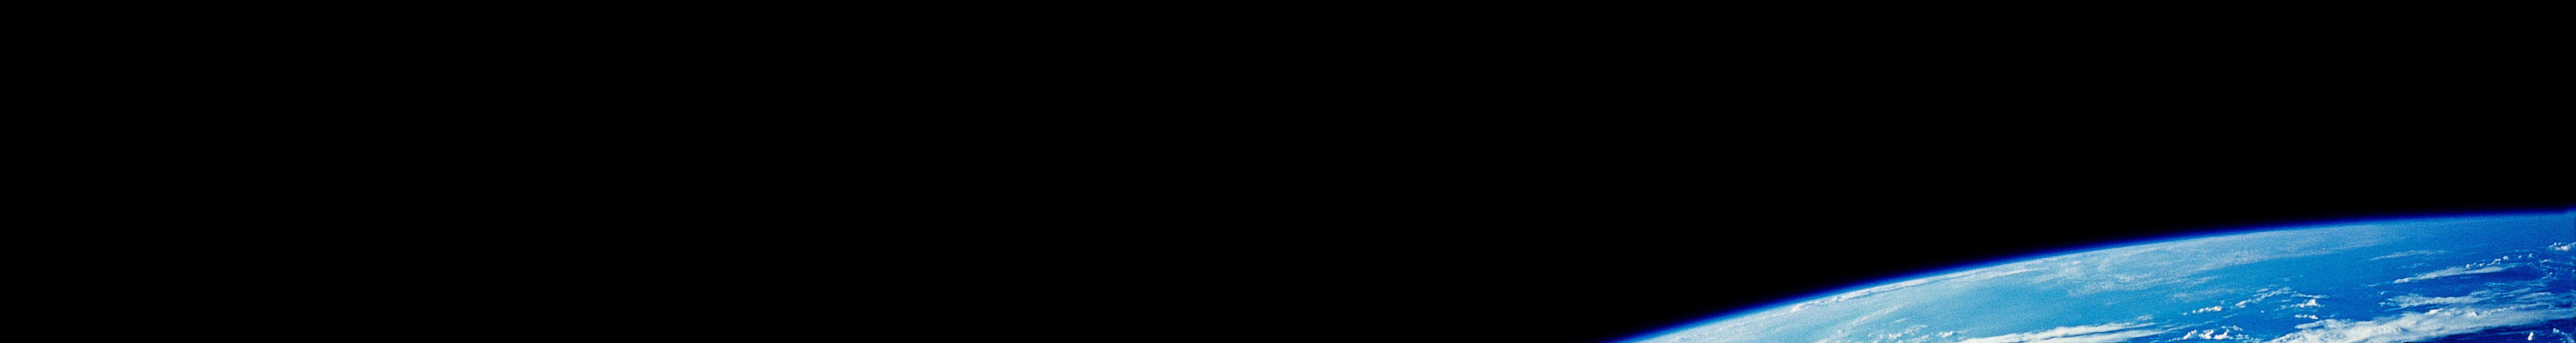
\includegraphics[width=\paperwidth]{figure/earth}}

\begin{document}
\begin{frame}[t]
  % Top title area
  \color{white} 
  \vspace*{2cm}
  \begin{columns}
    \begin{column}[t]{.97\textwidth}
      {\bfseries\fontsize{88}{120}\selectfont \inserttitle}
      {\fontsize{88}{120}\selectfont\kern2cm---\kern2cm\insertsubtitle}
    \end{column}
  \end{columns}

  \vspace*{2cm}
  \begin{columns}
    \begin{column}[t]{.2\textwidth}
      {\fontsize{45}{45}\selectfont\insertauthor\\[0.5cm]
        \fontsize{42}{42}\selectfont{\itshape\insertinstitute}\\[0.1cm]
        \fontsize{30}{30}\selectfont\texttt{\,\contact}}
      \vspace*{3cm}
    \end{column}

    \begin{column}[t]{.5\textwidth}
      {\fontsize{36}{42}\selectfont\setlength{\parskip}{36pt}At the Norwegian Mapping Authority, we are currently developing Where, a new
software for geodetic analysis. Where is built on our experiences with the
Geosat software, and will be able to analyse and combine data from VLBI, SLR,
GNSS and DORIS. The software is mainly written in Python which has proved very
fruitful. The code is quick to write and the architecture is easily extendable
and maintainable, while at the same time taking advantage of well-tested libraries
like the SOFA and IERS packages.

At the moment the VLBI analysis is close to ready. Comparison to other softwares
show that theoretical delay computations in Where are consistent with those. SLR
and GNSS analysis is well under way.

\vspace*{-10cm}

\endinput
}
    \end{column}
    
    \begin{column}[t]{.2\textwidth}
      \raisebox{-10.5cm}{\kern25cm\color{white}\tiny PHOTO: GETTY IMAGES}
      \vspace*{-10.5cm}
    \end{column}
  \end{columns}

  \begin{columns}

  % Left image column
    \begin{column}[t]{.12\textwidth}
      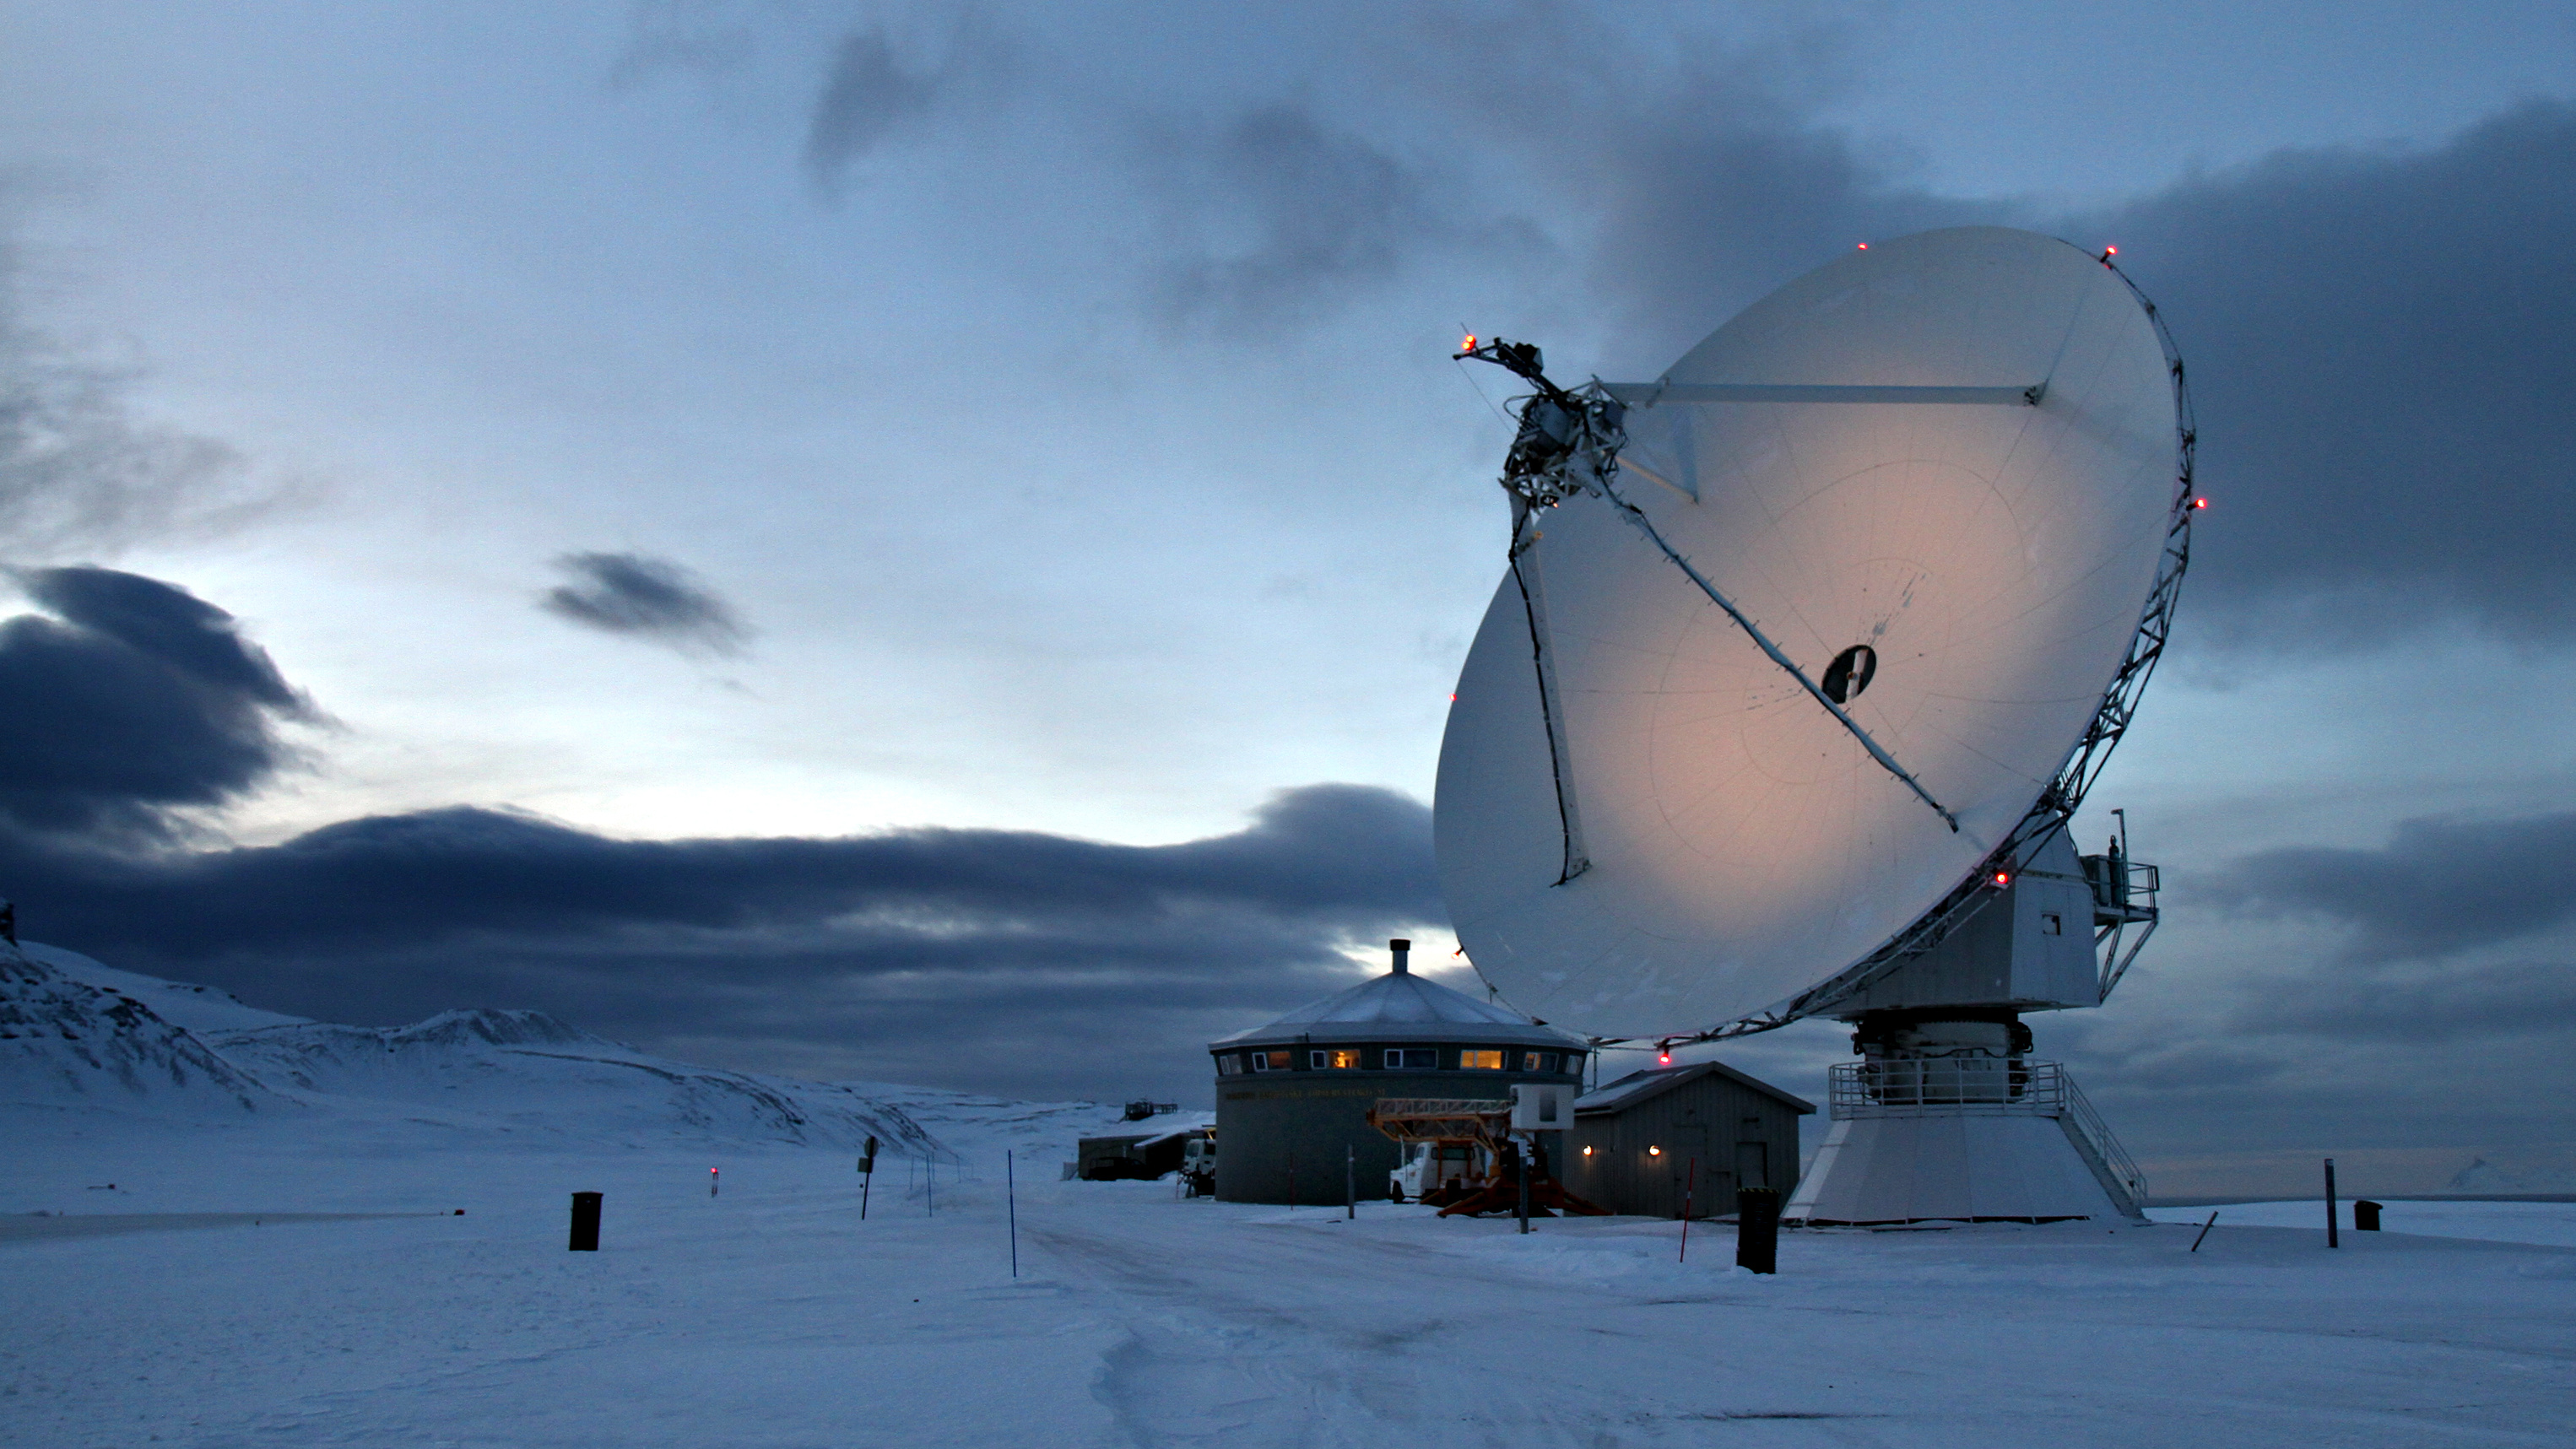
\includegraphics[width=\textwidth]{figure/vlbi}
      \raisebox{0.2cm}{\kern-6.8cm\color{white}\tiny PHOTO: BJ{\O}RN-OWE HOLMBERG}
      \vskip-1ex
      \begin{block}{VLBI}
        \vskip-3.3ex
      \end{block}

      \vspace*{1cm}
      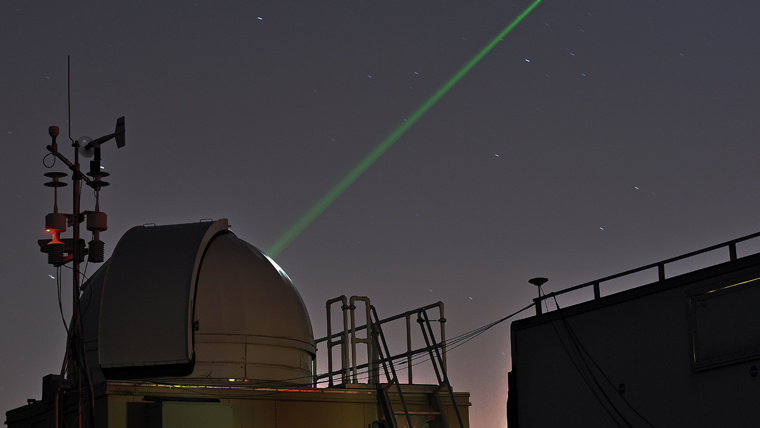
\includegraphics[width=\textwidth]{figure/slr}
      \raisebox{0.2cm}{\kern-5.8cm\color{white}\tiny PHOTO: FELIPE HALL / HTSI}
      \vskip-1ex
      \begin{block}{SLR}
        \vskip-3.3ex
      \end{block}

      \vspace*{1cm}
      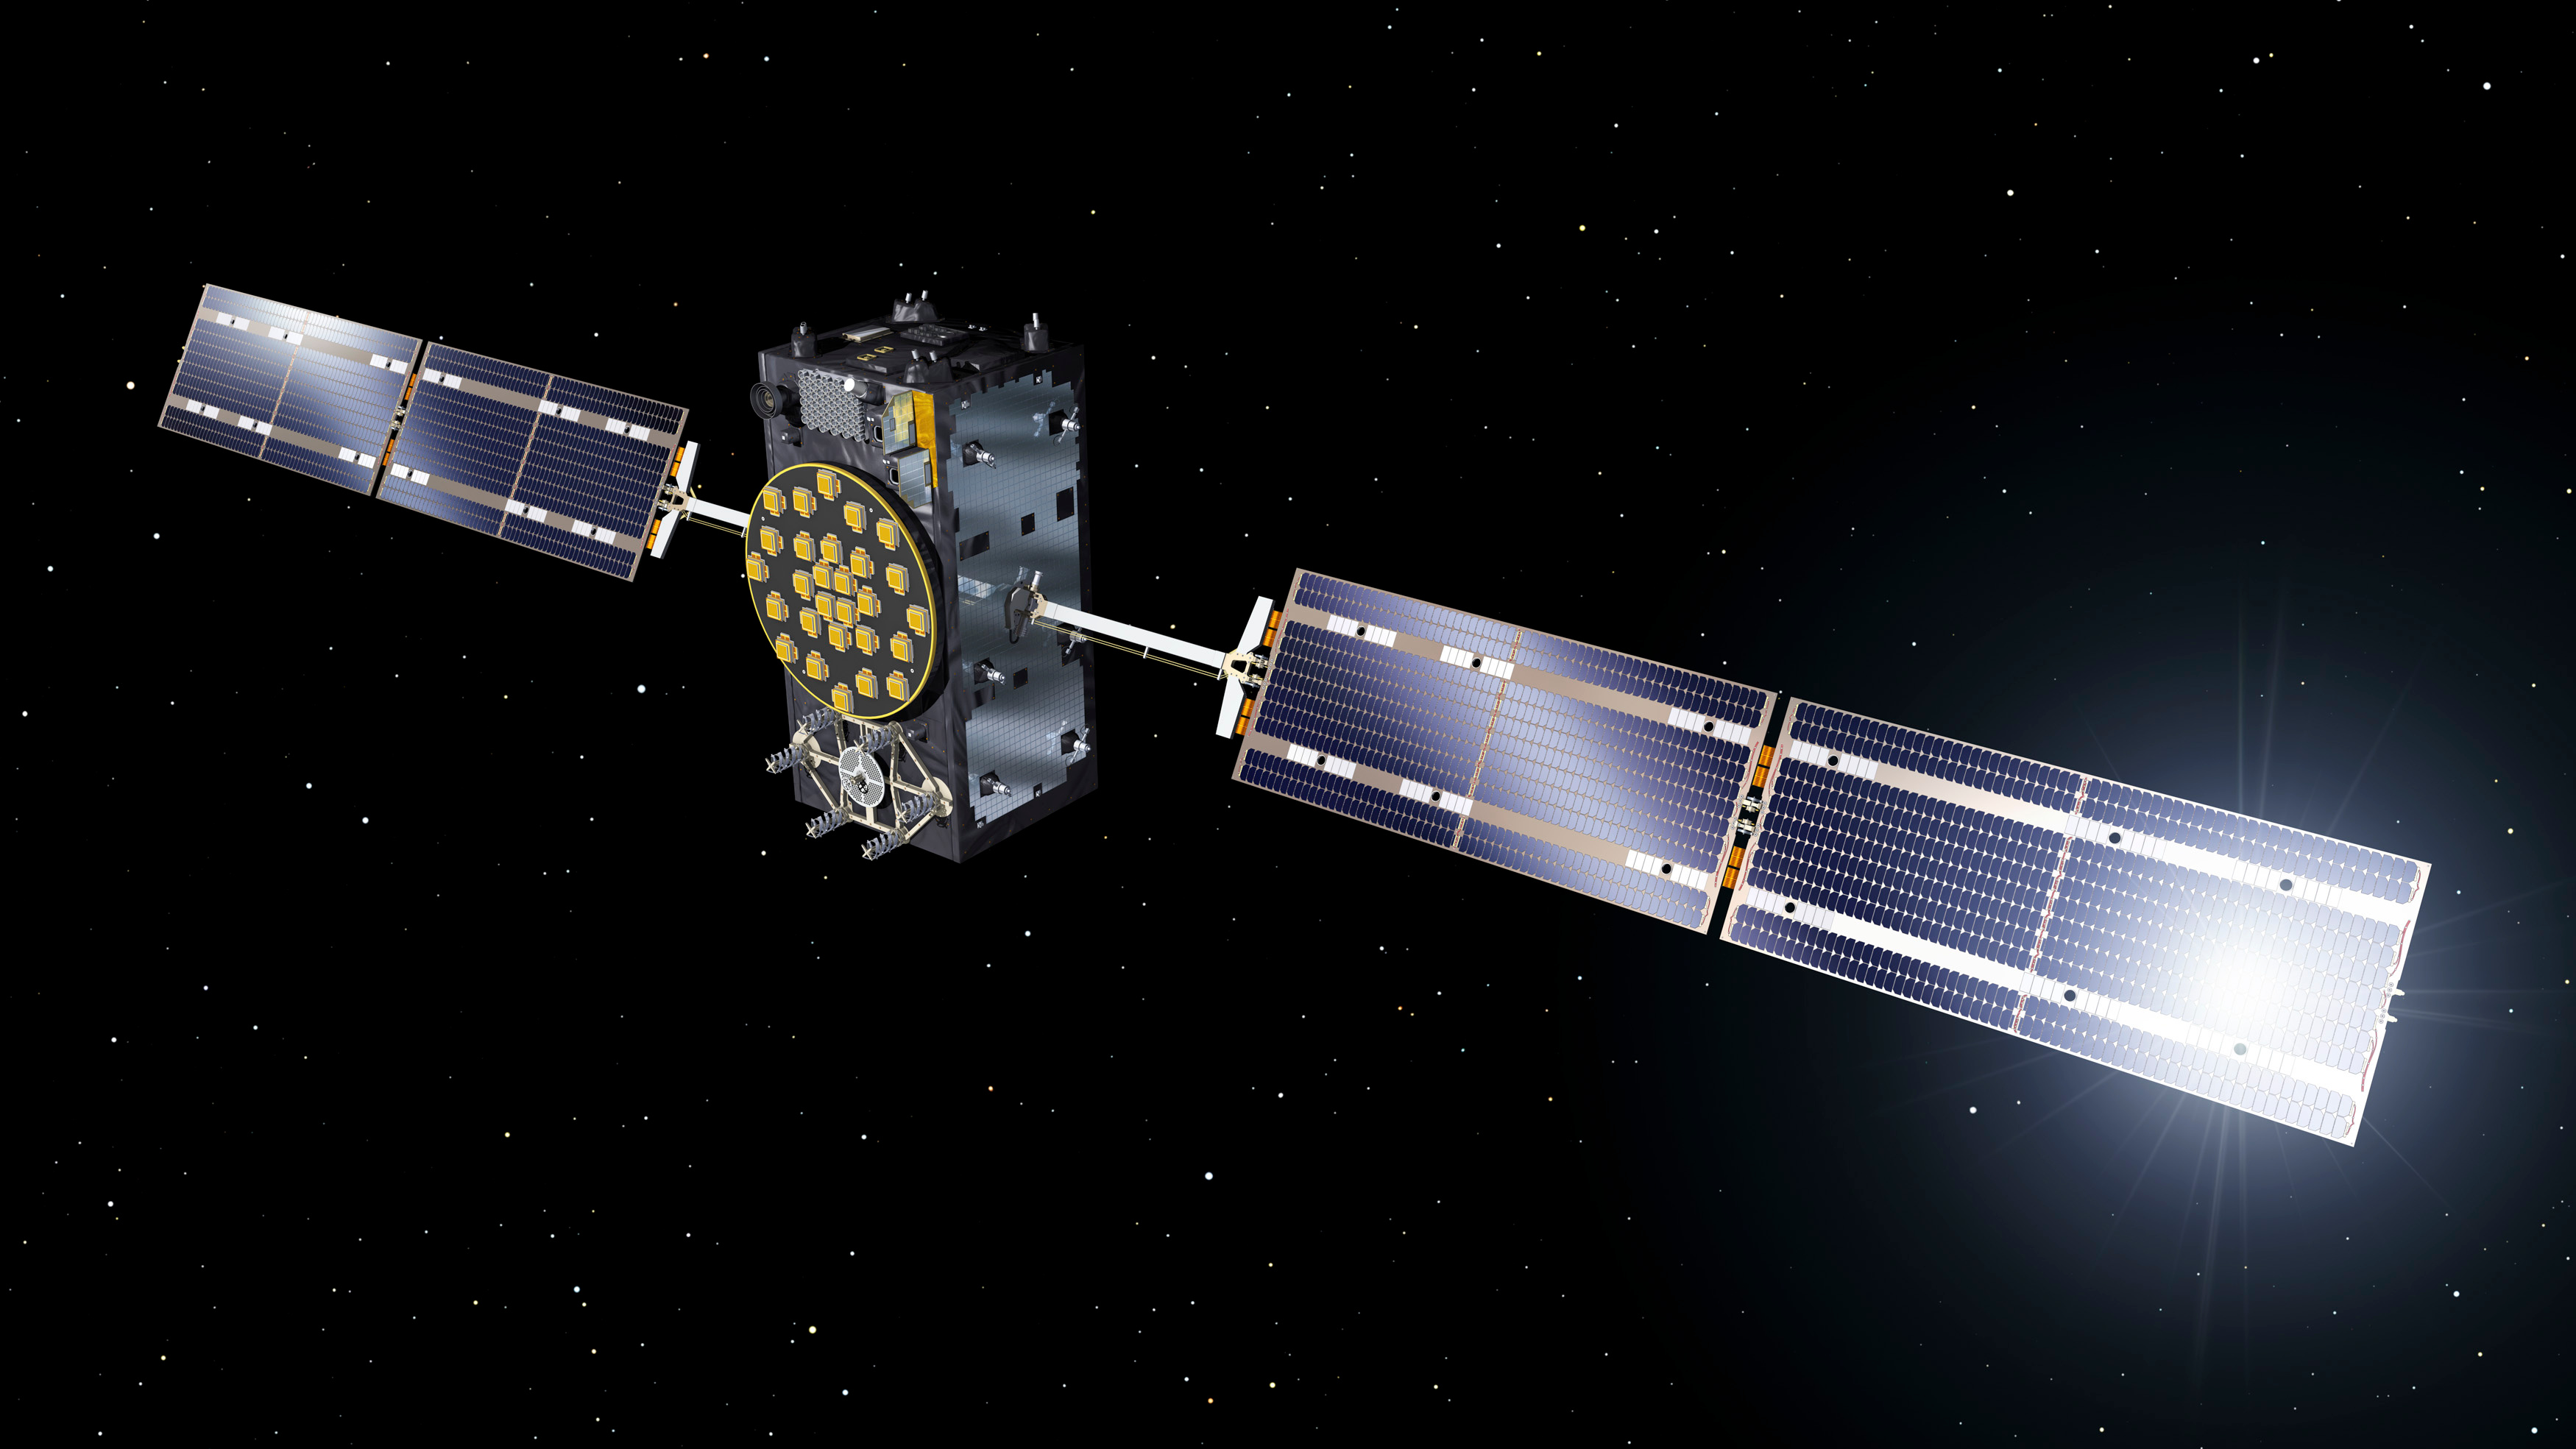
\includegraphics[width=\textwidth]{figure/gnss}
      \raisebox{0.2cm}{\kern-5cm\color{white}\tiny PHOTO: ESA -- J. HUART}
      \vskip-1ex
      \begin{block}{GNSS}
        \vskip-3.3ex
      \end{block}

      \vspace*{1cm}
      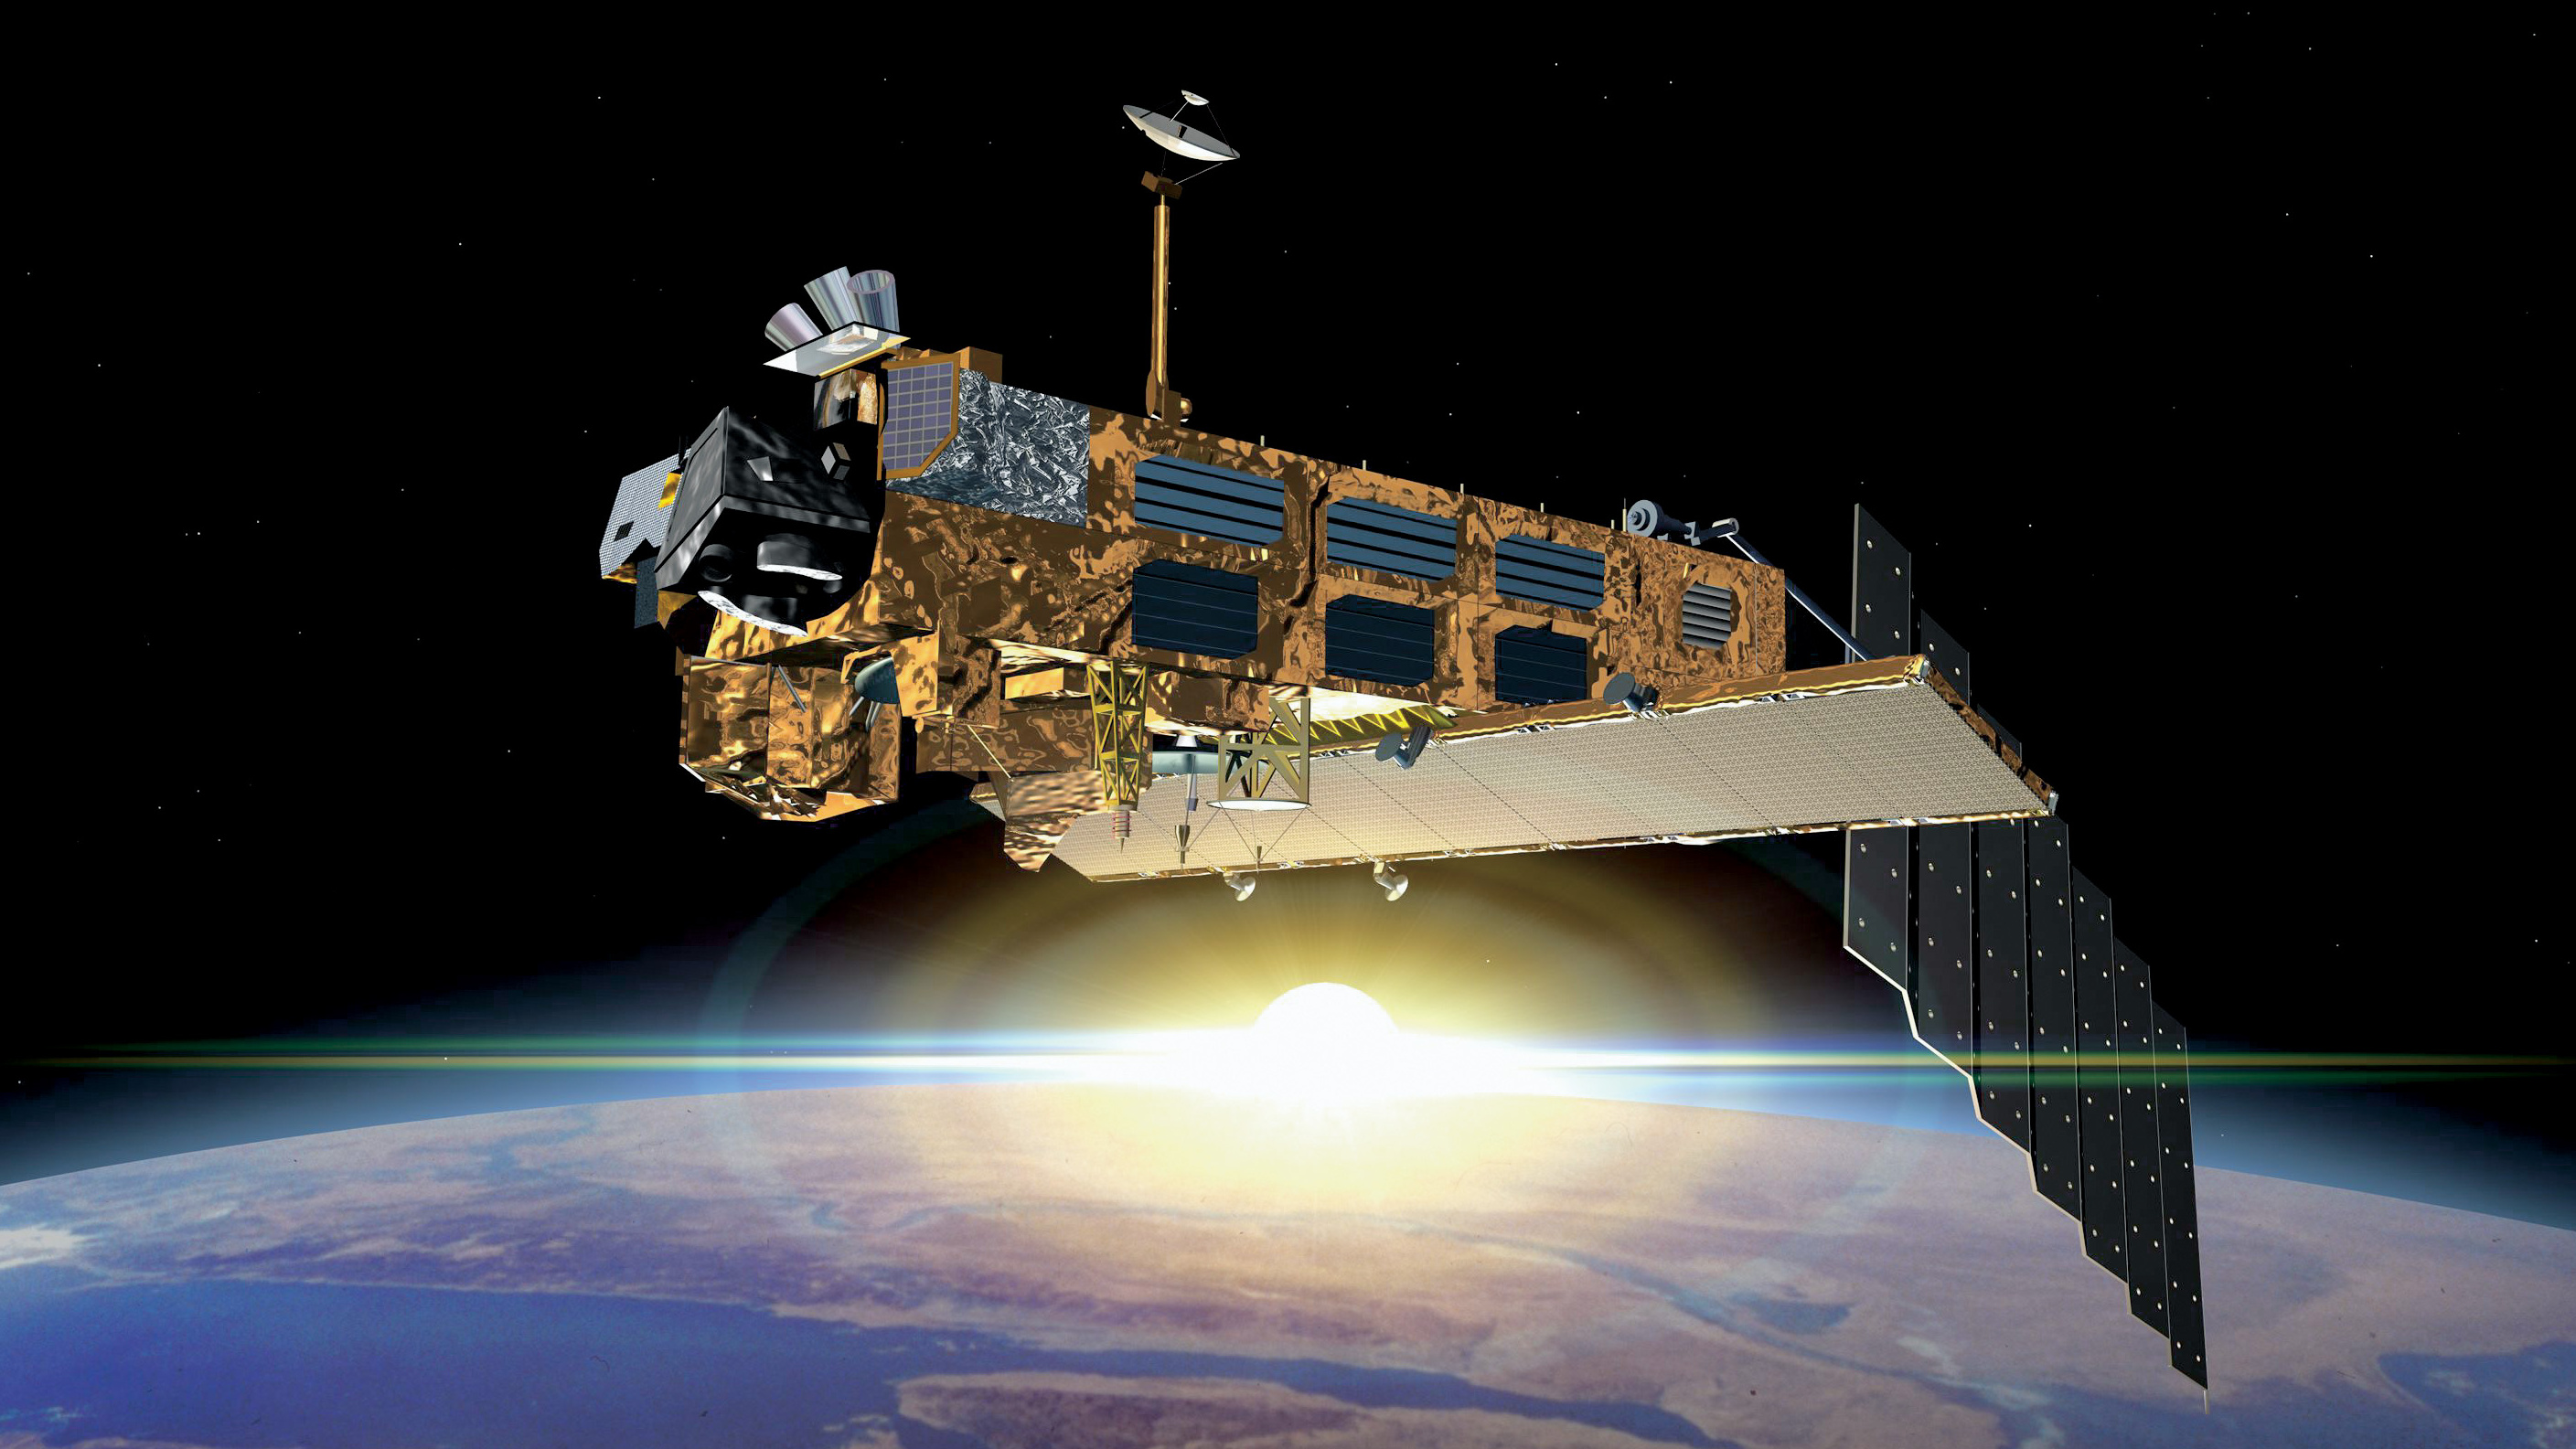
\includegraphics[width=\textwidth]{figure/doris}
      \raisebox{0.2cm}{\kern-8.3cm\color{white}\tiny PHOTO: ESA -- DENNMAN PRODUCTIONS}
      \vskip-1ex
      \begin{block}{DORIS}
        \vskip-3.3ex
      \end{block}
    \end{column}

    % Content area
    \begin{column}[t]{.26\textwidth}
      \vspace*{-6cm}
      \begin{block}{Where}
        \begin{multicols}{2}
          \documentclass[12pt, english]{beamer}

% Packages
\usepackage{xcolor}
\usepackage{eulervm}
\usepackage[utf8]{inputenc}

% Theme
\mode<presentation>
{
  \usetheme{Honefoss}
  \setbeamertemplate{blocks}[rounded]
}

\newcommand{\comment}[1]{{\slshape\color{kvred}#1}}

\title{Where}
\subtitle{A Geodetic Software}
\author{Ingrid Fausk, Michael Dähnn, Ann-Silje Kirkvik}
\date{April 6, 2019}

\begin{document}
\frame[plain]{\titlepage}

\begin{frame}{Where Timeline}
  \begin{itemize}
    \item 2015: Start
    \item 2018: First release as an open source project on GitHub
    \item 2019: Two proposed IVS analysis centers with Where: 
       \begin{itemize}
         \item Kartverket, Norway
         \item Instituto Geográfico Nacional, Spain
       \end{itemize}
    \item 2020: IVS Analysis centers with Where?
    \item 2022: ILRS Analysis center with Where?
  \end{itemize}
\end{frame}

\begin{frame}{Live Demo of Where}
  \begin{itemize}
    \item Running \emph{Where}
    \item Running \emph{There}, a companion tool for visualizing results
    \item Status, discussion
    \item Bugs...
  \end{itemize}
  \begin{figure}
    \begin{flushleft}
      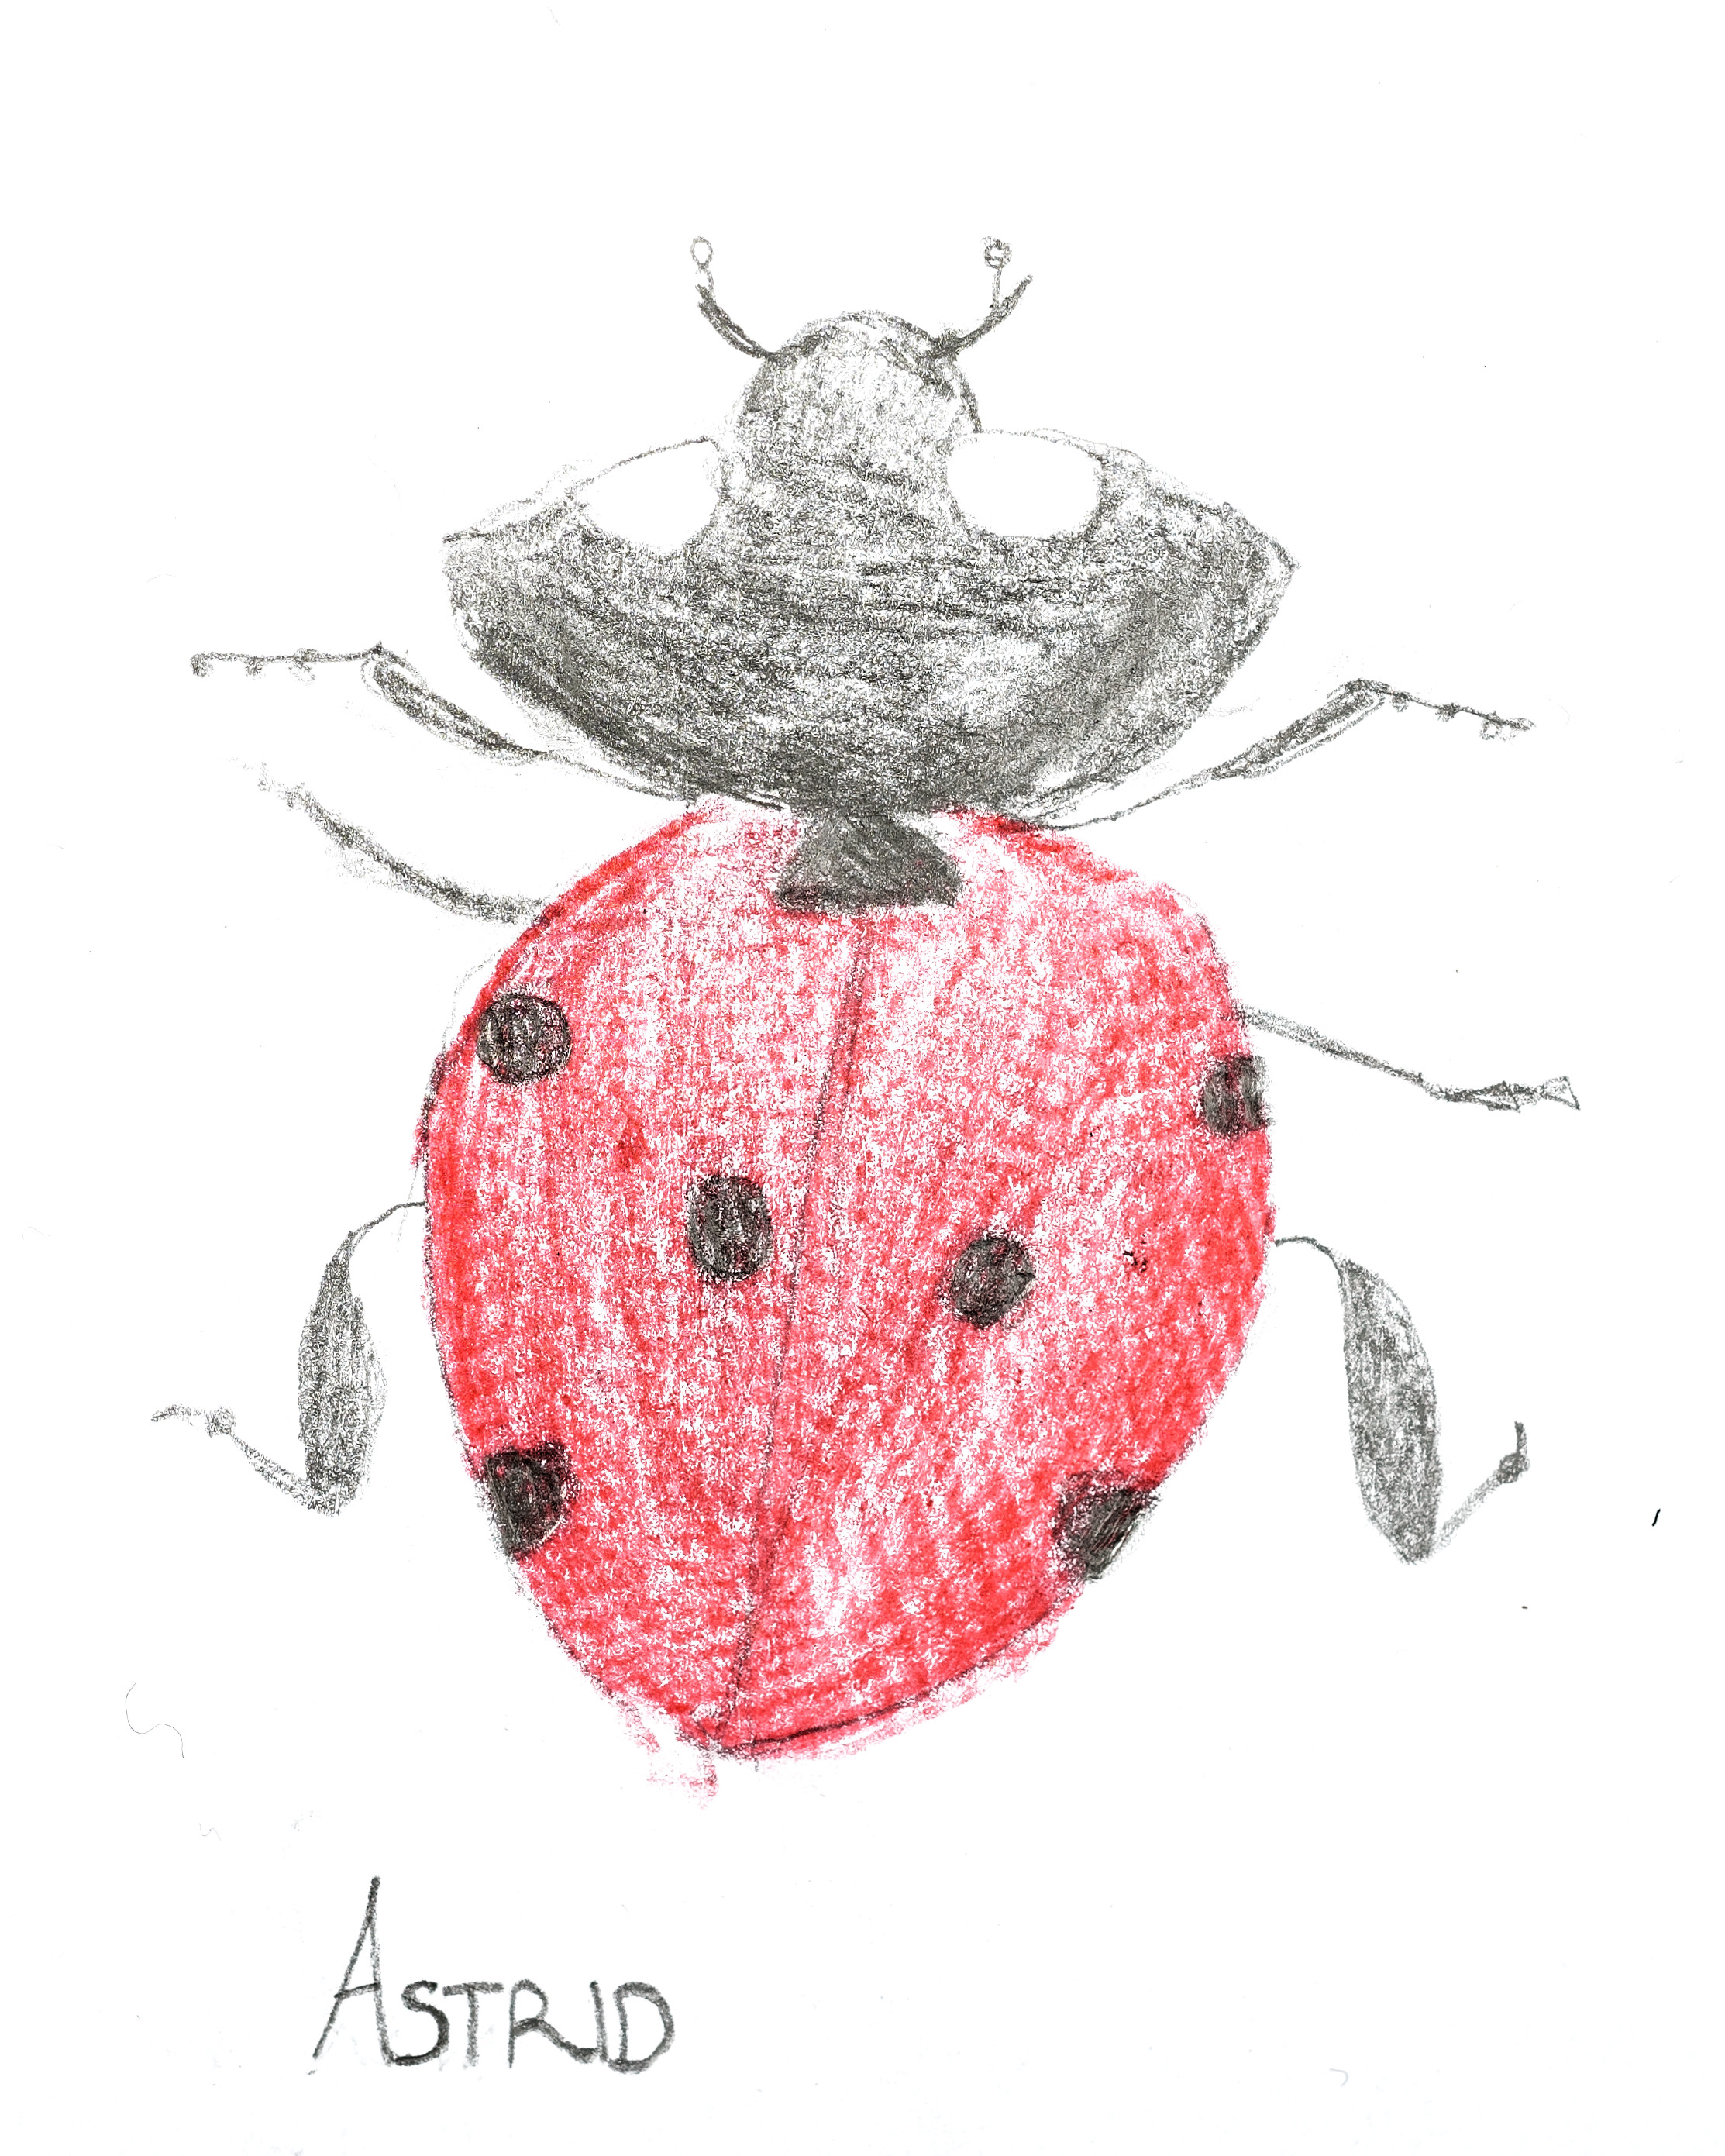
\includegraphics[width=2.5cm]{bug.jpg}
    \end{flushleft}
  \end{figure}     
\end{frame}

\begin{frame}{The Technical Stuff}

The \textbf{Where} software is mainly being written in \emph{Python}

  \begin{itemize}
    \item Cross-platform: Runs on Linux, Mac, Windows
    \item Solid, flexible and fast libraries like \texttt{numpy}, \texttt{astropy}, \texttt{matplotlib} and \texttt{scipy} are available
    \item We use a \textbf{HDF5}-based format for internal data storage
    \item \emph{Python} has effective interfaces to \emph{C} and \emph{Fortran} code, and we use the \textbf{SOFA} and \textbf{IERS} software libraries directly
    \item Orbit integrator using \emph{Cowell} method written in \emph{Python}. 
  \end{itemize}
\end{frame}

\end{document}

        \end{multicols}
      \end{block}
    \end{column}

    \begin{column}[t]{.52\textwidth}
      \begin{columns}
        \begin{column}[t]{.72\textwidth}
          \vspace*{-7cm}
          \begin{block}{Comparison to current softwares}
            \begin{multicols}{3}
              In 2015 and 2016 Grzegorz Klopotek carried out a VLBI Analysis Software
Comparison Campaign (VASCC). The goal of the campaign was to compare computed
theoretical delays from different software packages. In total 11 different
software packages contributed to the campaign and the results where presented at
the IVS General Meeting in South Africa in 2016~\cite{klopotek2016}.

The Norwegian Mapping Authority provided solutions to VASCC using the legacy
software GEOSAT~\cite{kierulf2010}. However, as development of the new software
progressed we redid the analysis from the VASCC campaign using Where and
compared the results with the computed theoretical delays from the
c5++~\cite{hobiger2010} and VieVS~\cite{boehm2012} softwares.

The VASCC dataset includes two networks of stations: one with four stations on
the southern hemisphere (SH) and one with five stations on the northern
hemisphere (NH).  Virtual observations of one radio source for each network are
scheduled every minute for 15 days, from June 22nd to July 7th 2015. A leap
second is introduced at midnight June 30th.

The VASCC delay model includes geometric and gravitational delay from the IERS
2010 Conventions~\cite{iers2010}. Also the delay through the
troposphere~\cite{iers2010} (hydrostatic delay with GMF mapping function) and
delay due to thermal deformations (with constant temperatures) and axis offset
as described by~\cite{nothnagel2009} are included. Delays due to cable
calibration, the ionosphere and clocks are ignored. Site displacement models
includes solid earth tides, solid earth pole tides, ocean tidal loading
(FES2004) and ocean loading pole tides according to~\cite{iers2010}. The version
of the IERS Conventional mean pole model used in VASCC is 2010. Atmospheric
pressure loading and eccentricity vectors are ignored. The apriori EOP time
series is corrected for ocean tides and liberation effects with periods less
than two days according to~\cite{iers2010}.

In the original campaign six software packages got sub-millimeter agreement when
comparing the RMS of the difference in theoretical delays. The absolute value of
the largest difference in residual was 2.68~mm and the smallest difference was
0.83~mm. The solution from two of the these six software packages,
c5++~\cite{hobiger2010} and VieVS~\cite{boehm2012}, were compared with Where and
the results are summarized in tables~\ref{tbl:vascc_rms}
and~\ref{tbl:vascc_max}. Figures~\ref{fig:where_c5++_sh}, \ref{fig:where_vievs_sh}
and~\ref{fig:c5++_vievs_sh} show the difference between Where, c5++ and VieVS
for the southern network.

These results indicate that the VLBI delay model in Where is consistent with
existing software packages and current conventions. The VASCC dataset
has been valuable in the development and testing of Where. An extension of the
campaign to include for instance the VMF1 mapping function and partial
derivatives would also be useful.

\endinput

            \end{multicols}
          \end{block}

          \vspace*{2cm}
          \begin{table}
            \color{black}
\begin{tabularx}{\columnwidth}{l|X}
  EOP & Lagrange interpolation with correction models: Tidal deformation,
  Subdaily tides, Polar motion due to long period ocean tides \\
  \hline
  Orbit models & Earth gravity field (with Solid Earth and Ocean Tides),
  Gravity field of Sun, Moon and planets, Solar radiation, Indirect solar radiation,
  Drag, Relativistic effects, Empirical forces \\
  \hline
  Ephemerides & DE405, DE421, DE430 \\
  \hline
  Displacement models & Atmospheric loading, Eccentricity vector, Ocean loading,
  Ocean pole tides, Solid Earth tides, Solid Earth pole tides \\
  \hline
  Troposphere & GMF, GPT, GPT2, GPT2w, VMF1 \\
  \hline
  VLBI models & Axis offset, Cable calibration, Geometric delay, Gravitational
  delay, Ionosphere, Thermal deformation \\
  \hline
  GNSS models & Antenna correction, Carrier phase wind-up, Ionosphere (higher
  order), Relativistic effects, Range \\
  \hline
  Estimation & Continuous piecewise linear Kalman Filter: Clock, EOP (Polar
  motion, $\Delta$UT1, Nutation), Source direction, Station position, Troposphere
  (Wet delay, Gradients)
\end{tabularx}

\endinput

            \caption{Models and apriori data supported by Where}
            \label{tbl:models}
          \end{table}
        \end{column}

        \begin{column}[t]{.03\textwidth}
          % spacing
        \end{column}
        
        \begin{column}[t]{.24\textwidth}
          \vspace*{-7cm}
          \begin{block}{References}
            \footnotesize
\bibliographystyle{../../where}
\bibliography{../../where}
\endinput

          \end{block}
        \end{column}
      \end{columns}

      % Figure strip
      \vspace*{1cm}
      \begin{columns}
        \begin{column}[t]{.24\textwidth}
          \begin{figure}
            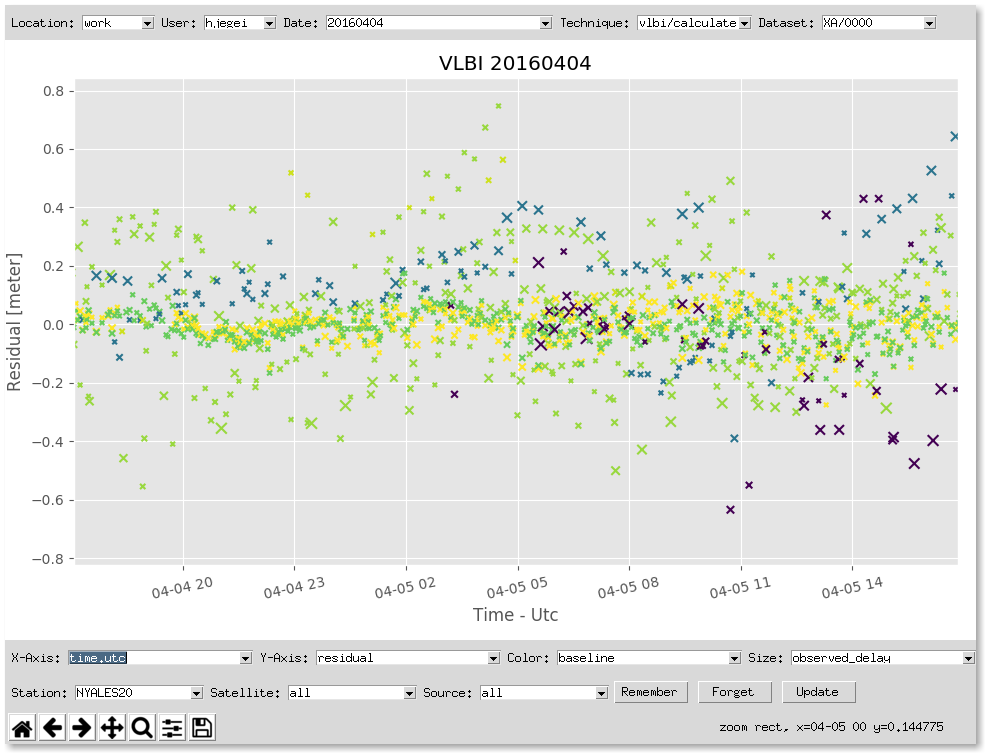
\includegraphics[width=\textwidth]{figure/there}
            \caption{A screenshot of There. There is a graphical tool developed
              to look into the results and analysis done by Where.}
            \label{fig:there}
          \end{figure}
        \end{column}

        \begin{column}[t]{.24\textwidth}
          \begin{figure}
            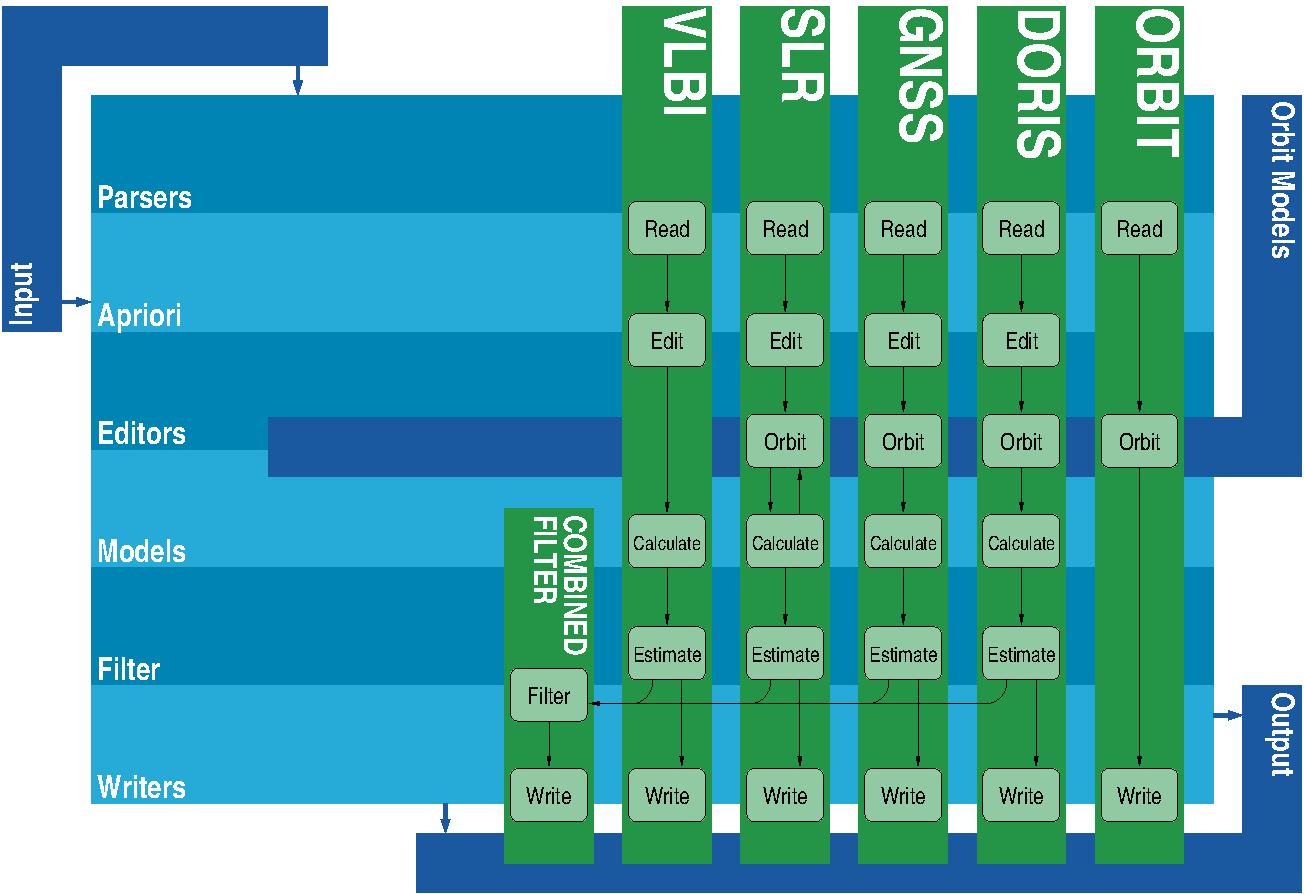
\includegraphics[width=\textwidth]{figure/code_structure}
            \caption{An overview of the architecture of Where. The pipeline for
              the analysis of the different techniques, as well as orbit
              determination and combination of different techniques is shown.}
            \label{fig:architecture}
          \end{figure}
        \end{column}

        \begin{column}[t]{.24\textwidth}
          \begin{figure}
            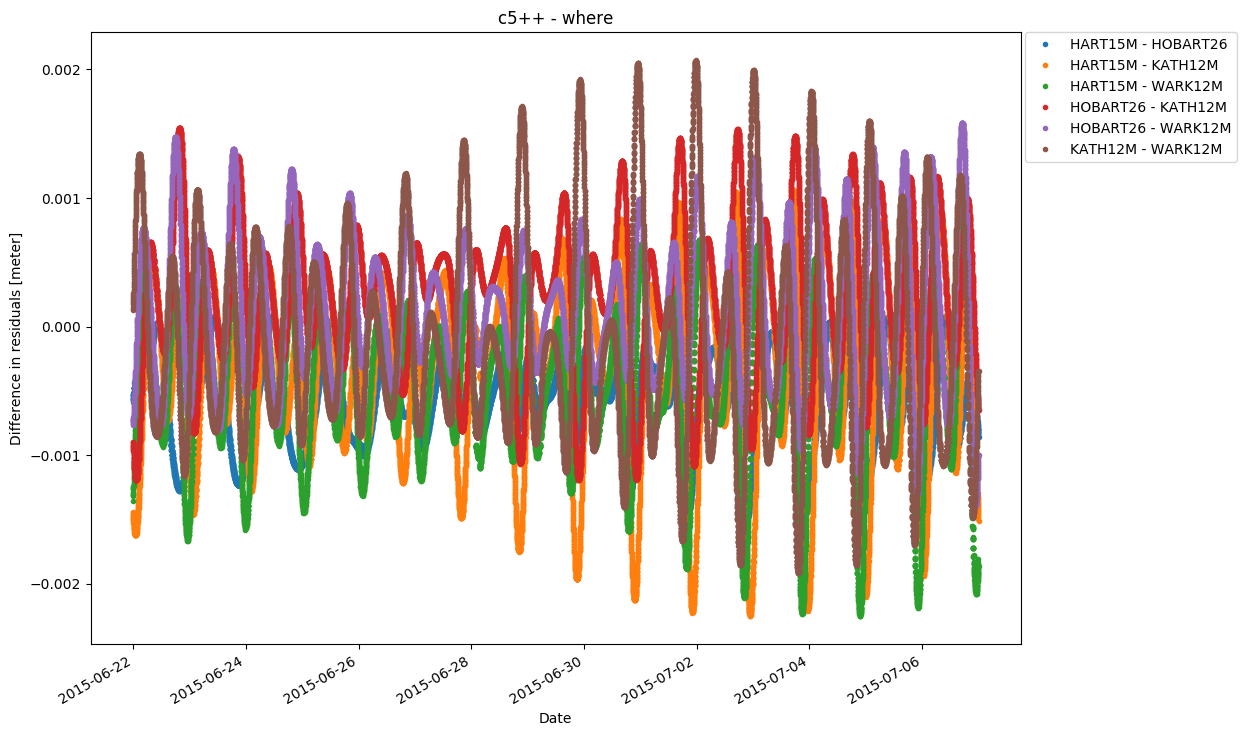
\includegraphics[width=\textwidth]{figure/c5++_vs_where_SH}
            \caption{Difference in theoretical delay between c5++ and Where for
              each baseline in the southern network used in the VASCC. The RMS
              of all differences is 0.72~mm.}
            \label{fig:c5_where_sh}
          \end{figure}
        \end{column}

        \begin{column}[t]{.24\textwidth}
          \begin{figure}
            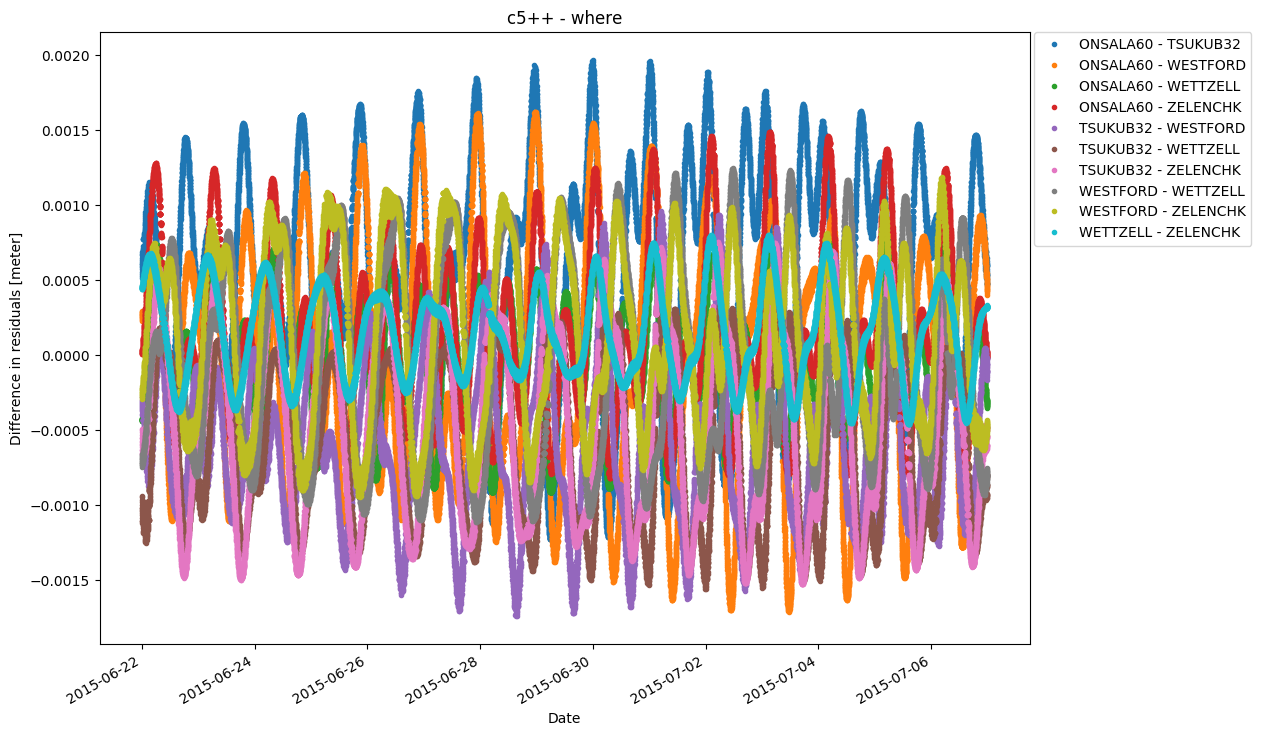
\includegraphics[width=\textwidth]{figure/c5++_vs_where_NH}
            \caption{Difference in theoretical delay between c5++ and Where for
              each baseline in the northern network used in the VASCC. The RMS
              of all differences is 0.68~mm.}
            \label{fig:c5_where_nh}
          \end{figure}
        \end{column}
      \end{columns}
    \end{column}

  \end{columns}
\end{frame}
\end{document}
